%Radio description
{\Large Radio Bands}
%Draw a sinewave with
%	{Initial Amplitude x.xxx}{Initial Time-width x.xxx}{Initial Number of cycles x}
%	{Second Amplitude x.xxx}{Second Time-width x.xxx}{Second Number of cycles x}
%	{Total repeats}
\newlength{\nAmplitude}		\newlength{\nAmplitudeNeg}
\newlength{\nTime}		\newlength{\nTimeTwo}		\newlength{\nTimeThree}		\newlength{\nTimeFour}
\newlength{\nSAmplitude}	\newlength{\nSAmplitudeNeg}
\newlength{\nSTime}		\newlength{\nSTimeTwo}		\newlength{\nSTimeThree}	\newlength{\nSTimeFour}
\newlength{\nTimeEnd}		\newlength{\nSTimeEnd}		\newlength{\nSTimeStart}
\newcommand{\sinewave}[7]{
	\setlength{\nAmplitude}{#1}
	\setlength{\nAmplitudeNeg}{\nAmplitude*-1}
	\setlength{\nTime}{#2}
	\setlength{\nTimeTwo}{\nTime*2}
	\setlength{\nTimeThree}{\nTime*3}
	\setlength{\nTimeFour}{\nTime*4}
	\setlength{\nTimeEnd}{\nTime*4*#3}
	\setlength{\nSAmplitude}{#4}
	\setlength{\nSAmplitudeNeg}{\nSAmplitude*-1}
	\setlength{\nSTime}{#5}
	\setlength{\nSTimeTwo}{\nSTime*2}
	\setlength{\nSTimeThree}{\nSTime*3}
	\setlength{\nSTimeFour}{\nSTime*4}
	\setlength{\nSTimeEnd}{\nTime*4*#3+\nSTime*4*#6}
	\multido{\dXTimePosition=0.000in+\nSTimeEnd}{#7}{
		\multido{\dXPosition=\dXTimePosition+\nTimeFour}{#3}{
			\rput(\dXPosition,0){
			\parabola(0.00,0)(\nTime,\nAmplitude)\parabola(\nTimeTwo,0)(\nTimeThree,\nAmplitudeNeg)
			}
		}
		\setlength{\nSTimeStart}{\dXTimePosition+\nTimeEnd}
		\multido{\dXPosition=\nSTimeStart+\nSTimeFour}{#6}{
			\rput(\dXPosition,0){
			\parabola(0.00,0)(\nSTime,\nSAmplitude)\parabola(\nSTimeTwo,0)(\nSTimeThree,\nSAmplitudeNeg)
			}
		}
	}
}
%

% None: f(x) = sin(20x)
% AM: f(x) = cos(.5x)∙sin(20∙x)
% FM: f(x) = cos(20∙x+15∙sin(x))


% Preamble: 
% \pgfplotsset{width=7cm,compat=1.14}
% \begin{tikzpicture}
% \begin{axis}[
% hide x axis,
% hide y axis
% ]
% \addplot [red]{sin(deg(x))};
% \addplot [green]{cos(deg(x))};
% \end{axis}

% \begin{axis}[enlarge x limits=false]
% \addplot [red,samples=500] {sin(deg(x))};
% \addplot [orange,samples=7] {sin(deg(x))};
% \addplot [teal,const plot,samples=14]
% {sin(deg(x))};
% \end{axis}
% \end{tikzpicture}% <- eliminate space.
% \end{document}

% None: f(x) = sin(20x)
% AM: f(x) = cos(.5x)∙sin(20∙x)
% FM: f(x) = cos(20∙x+15∙sin(x))

\pgfplotsset{%
	axis line style={draw=none},
	tick style={draw=none},
	xticklabels=\empty,
	yticklabels=\empty,
	domain=0:3*pi,
	samples=1e3,
	width=2.3in,
	height=1in,
	xlabel shift=-8pt,
}

\begin{itemize}

%Country flags from here (using MIT license):
% https://github.com/stevenrskelton/flag-icon
% use inkscape to convert to eps which is smaller than using "convert"
%
%List of telecommunications regulatory bodies
% https://en.wikipedia.org/wiki/List_of_telecommunications_regulatory_bodies
% 
\item {%
\setlength{\fboxsep}{0pt}%
\setlength{\fboxrule}{0.5pt}%
The radio spectrum (ELF to EHF) is populated by many more items than can be shown on this chart. Only a small sampling of the bands used around the world are shown. Each country has its own rules and regulations for allotting bands in this region. FCC \fbox{
\includegraphics[width=0.15in]{tex/us.eps}}, CRTC \fbox{
\includegraphics[width=0.15in]{tex/ca.eps}}, OFCOM \fbox{
\includegraphics[width=0.15in]{tex/gb.eps}}, BNA  \fbox{
\includegraphics[width=0.15in]{tex/de.eps}}, CII  \fbox{
\includegraphics[width=0.15in]{tex/cn.eps}}...
}%
\item Communication by EMR is done by modulating the carrier waveform:

\begin{tabular}{ccc}%
\begin{tikzpicture} % No modulation
	\begin{axis}[smooth,grid=none,scale=1,xlabel={No modulation},line width=1pt,]
		\addplot[white, smooth,xlabel={No modulation},line join=round, line cap=round] {sin(x*20*180/pi)};
	\end{axis}
\end{tikzpicture}&
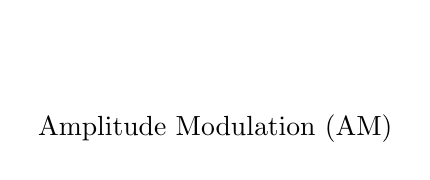
\begin{tikzpicture} %AM
	\begin{axis}[smooth,grid=none,scale=1,xlabel={Amplitude Modulation (AM)},line width=1pt,]
		%\addplot[white, smooth,line join=round, line cap=round] {sin(x*20*180/pi)*sin(x*1*180/pi)};
		\addplot[white, smooth,line join=round, line cap=round] {0.5*sin(x*20*180/pi)*(1+sin(x*1.7*180/pi))+8};

	\end{axis}
\end{tikzpicture}&
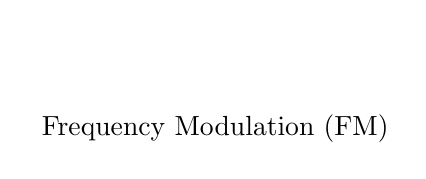
\begin{tikzpicture} % FM
	\begin{axis}[smooth,grid=none,scale=1,xlabel={Frequency Modulation (FM)},line width=1pt,]
		\addplot[white, smooth,line join=round, line cap=round] {sin((x*20 + 6*(sin(x*2*180/pi)))*180/pi)};
	\end{axis}
\end{tikzpicture}
\end{tabular}
%
% \item Not all references agree on the ULF band range, the HAARP range is used here.
%
\item {\bfseries RA}dio {\bfseries D}etecting {\bfseries A}nd {\bfseries R}anging (RADAR) uses microwaves to detect the distance and speed of objects.

\item {\bfseries C}itizens {\bfseries B}and Radio (CB) contains 40 stations between 26.965 - 27.405MHz %\hspace{0.02in}
{% CB Radio
  \definecolor{BoxColor}{rgb}{0.6,0.68,0.86}
  \psframebox[linestyle=none,framesep=1pt,fillcolor=BoxColor,linearc=0]{\black CB}
}.
%
 Schumann resonances are produced in the cavity between the Earth and the ionosphere \hspace{0.02in}%
 \psframebox[fillstyle=none,linestyle=none]{\psscalebox{0.7}{\blip{0,-.07}{S}}}%
 \hspace{0.02in}.
%
 Hydrogen gas emits radio band EMR at 21cm  \hspace{0.05in}%
 \psframebox[fillstyle=none,linestyle=none]{\psscalebox{0.7}{\blip{0,-.07}{H}}}%
 \hspace{0.02in}.
%
 Time / frequency standards shown as \psframebox[linestyle=none] {\rput(0.1in,0){\timestandard}} \hspace{0.1in}.
% 
 Other individual frequencies are represented as icons:\vspace{0.1in}\\
\begin{tabular}{cp{1.4in}cp{1in}cp{1.7in}}
% 
\psframebox[linestyle=none]{\submarine{0.02,.0}{xxHz}}\hspace{0.2in}\vspace{0.05in} & Submarine&
\psframebox[linestyle=none]{\rput(0.15,.05)\pager}&Pager&
\psframebox[linestyle=none]{\rput(0.05,.05){\psframebox[fillstyle=solid,fillcolor=Itinerant,linecolor=Itinerant,linearc=0,framesep=1pt]{\textcolor{Black}{GMRS}}}}&General Mobile Radio Service\\%
%
\psframebox[linestyle=none]{\rput(0.14,0.01){\psframebox[fillstyle=solid,fillcolor=green,linecolor=green,linearc=0]{\textcolor{Black}{xxm}}}}\hspace{.1in}\vspace{0.05in} & Ham / international&
\psframebox[linestyle=none]{\rput(0.14,.03){\weatherstation}\hspace{.03in}\vspace{0.08in}} & Weather&
\psframebox[linestyle=none]{\rput(0.15,.04){
	\psframe[linestyle=solid,linecolor=gray,fillstyle=solid,fillcolor=gray,linearc=0](-.2,-.08)(.2,.08)
	\psframe[hatchwidth=2pt, hatchsep=1.5pt,linestyle=solid,linecolor=yellow,fillstyle=hlines,hatchangle=45,hatchcolor=yellow,fillcolor=gray,linearc=0](-.2,-.08)(.2,.08)
	}
	\hspace{.2in}}\vspace{0.05in}
	& Short wave\\
%
%
\psframebox[linestyle=none]{\rput(0.11,.05){\psframebox[fillstyle=solid,fillcolor=Itinerant,linecolor=Itinerant,linearc=0,framesep=1pt]{\textcolor{Black}{FRS}}}}&Family Radio Service&
\psframebox[linestyle=none]{\rput(0.15,-0.1){\wirelessmic}}&Wireless Mic.&
\psframebox[linestyle=none]{
% 	\rput(0.15,.05){
% 		\psframebox[fillstyle=solid,linearc=0,linecolor=yellow,framesep=1pt,fillcolor=yellow,linewidth=1pt,linestyle=solid]{\textcolor{Black}{CP}}
% 	}
	\rput(0.08, 0.02){
		\psset{linestyle=solid, linewidth=0.02in}
		\psline[linecolor=cyan  ](-.15,0.04)(0.15,0.04)
		\psline[linecolor=green ](-.20,0.02)(0.10,0.02)
		\psline[linecolor=orange](-.10,0.00)(0.20,0.00)
	} 
	\hspace{.03in}\vspace{0.08in}} & Cellular Phones
	\psframebox[fillstyle=solid,linearc=0,linecolor=orange,framesep=1pt,fillcolor=orange,linewidth=1pt,linestyle=solid]{\textcolor{Black}{3G}}
	\psframebox[fillstyle=solid,linearc=0,linecolor=green, framesep=1pt,fillcolor=green, linewidth=1pt,linestyle=solid]{\textcolor{Black}{4G}}
	\psframebox[fillstyle=solid,linearc=0,linecolor=cyan,  framesep=1pt,fillcolor=cyan,  linewidth=1pt,linestyle=solid]{\textcolor{Black}{5G}}
\\
%
% \psframebox[linestyle=none]{
% 	\rput(0.11,.05){
% 		\psframebox[linestyle=none,framesep=1pt,fillcolor=red,linearc=0]{\white SOS}
% 	}
% }
% &
% 	\psset{dotsize=1pt 1}Distress signal, in Morse code:\vspace{0.18in}
% \rput(-1.4,-0.18){
% 	\rput(0,0.05){
% 		\psdots(0,0)(.1,0)(.2,0)\psline{cc-cc}(0.3,0)(0.42,0)\psline{cc-cc}(0.49,0)(0.61,0)\psline{cc-cc}(0.68,0)(0.8,0)\psdots(.9,0)(1,0)(1.1,0)
% 	}
% }%
\end{tabular}
% Slightly modified from this:
%   https://github.com/sikvall/latex-morse

\newcommand{\Mdotlength}{3pt}
\newcommand{\Mdahlength}{9pt}
\newcommand{\Mcharseplength}{9pt}
\newcommand{\Mwordseplength}{21pt}
\newcommand{\Mdiditlength}{6pt}
\newcommand{\Mfetvadd}{1.5pt}
\newcommand{\Mcharsep}{\hspace{9pt}}
\newcommand{\Mwordsep}{\hspace{21pt}}

\newcommand{\dit}{\raisebox{0.5ex}{$\rule{\Mdotlength}{\Mfetvadd}\hspace{\Mdotlength}$}}
\newcommand{\dah}{\raisebox{0.5ex}{$\rule{\Mdahlength}{\Mfetvadd}\hspace{\Mdotlength}$}}

\newcommand{\MCa}{\dit\dah            \Mcharsep}
\newcommand{\MCb}{\dah\dit\dit\dit  \Mcharsep}
\newcommand{\MCc}{\dah\dit\dah\dit   \Mcharsep}
\newcommand{\MCd}{\dah\dit\dit       \Mcharsep}
\newcommand{\MCe}{\dit                \Mcharsep} 
\newcommand{\MCf}{\dit\dit\dah\dit   \Mcharsep}
\newcommand{\MCg}{\dah\dah\dit      \Mcharsep}
\newcommand{\MCh}{\dit\dit\dit\dit   \Mcharsep}
\newcommand{\MCi}{\dit\dit            \Mcharsep}
\newcommand{\MCj}{\dit\dah\dah\dah   \Mcharsep}
\newcommand{\MCk}{\dah\dit\dah       \Mcharsep}
\newcommand{\MCl}{\dit\dah\dit\dit  \Mcharsep}
\newcommand{\MCm}{\dah\dah          \Mcharsep}
\newcommand{\MCn}{\dah\dit          \Mcharsep}
\newcommand{\MCo}{\dah\dah\dah        \Mcharsep}
\newcommand{\MCp}{\dit\dah\dah\dit  \Mcharsep}
\newcommand{\MCq}{\dah\dah\dit\dah \Mcharsep}
\newcommand{\MCr}{\dit\dah\dit      \Mcharsep}
\newcommand{\MCs}{\dit\dit\dit      \Mcharsep}
\newcommand{\MCt}{\dah                \Mcharsep}
\newcommand{\MCu}{\dit\dit\dah       \Mcharsep}
\newcommand{\MCv}{\dit\dit\dit\dah  \Mcharsep}
\newcommand{\MCw}{\dit\dah\dah     \Mcharsep}
\newcommand{\MCx}{\dah\dit\dit\dah  \Mcharsep}
\newcommand{\MCy}{\dah\dit\dah\dah   \Mcharsep}
\newcommand{\MCz}{\dah\dah\dit\dit    \Mcharsep}
\newcommand{\MCAke}{\dit\dah\dah\dit\dah \Mcharsep}
\newcommand{\MCArlig}{\dit\dah\dit\dah   \Mcharsep}
\newcommand{\MCOsten}{\dah\dah\dah\dit   \Mcharsep}
\newcommand{\MCUbel}{\dit\dit\dah\dah    \Mcharsep} % Tyskt Ü
\newcommand{\MCch}{\dah\dah\dah\dah      \Mcharsep} % Tyskt CH

\newcommand{\MPunkt}{\dit\dah\dit\dah\dit\dah           \Mcharsep}
\newcommand{\MSTOP}{\MPunkt}
\newcommand{\MComma}{\dah\dah\dit\dit\dah\dah           \Mcharsep}
\newcommand{\MQuestion}{\dit\dit\dah\dah\dit\dit     \Mcharsep}
\newcommand{\MSlash}{\dah\dit\dit\dah\dit          \Mcharsep}
\newcommand{\MHyphen}{\dah\dit\dit\dit\dit\dah     \Mcharsep}
\newcommand{\MPlus}{\dit\dah\dit\dah\dit          \Mcharsep}
\newcommand{\MColon}{\dah\dah\dah\dit\dit\dit \Mcharsep}
\newcommand{\MApostrophe}{\dit\dah\dah\dah\dah\dit \Mcharsep}
\newcommand{\MQuoteMarks}{\dit\dah\dit\dit\dah\dit \Mcharsep}
\newcommand{\MSOS}{\dit\dit\dit\dah\dah\dah\dit\dit\dit \Mcharsep}

\newcommand{\MRepetera}{\dit\dit\hspace{\Mdiditlength}\dit\dit \Mcharsep}
\newcommand{\MAmpersand}{\dit\dah\dit\dit\dit                     \Mcharsep}
\newcommand{\MAtSign}{\dit\dah\dah\dit\dah\dit            \Mcharsep}
\newcommand{\MEquals}{\dah\dit\dit\dit\dah                \Mcharsep}
\newcommand{\MFelskrivning}{\dit\dit\dit\dit\dit\dit\dit\dit  \Mcharsep}

\newcommand{\MCone}{\dit\dah\dah\dah\dah   \Mcharsep}
\newcommand{\MCtwo}{\dit\dit\dah\dah\dah	  \Mcharsep}
\newcommand{\MCthree}{\dit\dit\dit\dah\dah   \Mcharsep}
\newcommand{\MCfour}{\dit\dit\dit\dit\dah  \Mcharsep}
\newcommand{\MCfive}{\dit\dit\dit\dit\dit   \Mcharsep}
\newcommand{\MCsix}{\dah\dit\dit\dit\dit   \Mcharsep}
\newcommand{\MCseven}{\dah\dah\dit\dit\dit   \Mcharsep}
\newcommand{\MCeight}{\dah\dah\dah\dit\dit  \Mcharsep}
\newcommand{\MCnine}{\dah\dah\dah\dah\dit   \Mcharsep}
\newcommand{\MCzero}{\dah\dah\dah\dah\dah  \Mcharsep}

\newcommand{\MWord}{\MWS}

\lstset{%
literate={A}{\MCa}1
%          {b}{\MBertil}1
%          {c}{\MCesar}1
%          {d}{\MDavid}1
%          {e}{\MErik}1
%          {f}{\MFilip}1
%          {g}{\MGustav}1
%          {h}{\MHelge}1
%          {i}{\MIvar}1
%          {j}{\MJohan}1
%          {k}{\MKalle}1
%          {l}{\MLudvig}1
%          {m}{\MMartin}1
%          {n}{\MNiklas}1
         {O}{\MCo}1
%          {p}{\MPetter}1
%          {q}{\MQvintus}1
%          {r}{\MRudolf}1
         {S}{\MCs}1
%          {t}{\MTore}1
%          {u}{\MUrban}1
%          {v}{\MViktor}1
%          {w}{\MWilhelm}1
%          {x}{\MXerxes}1
%          {y}{\MYngve}1
%          {z}{\MZata}1
         {å}{\MAke}1
         {ä}{\MArlig}1
         {ö}{\MOsten}1
         {.}{\MPunkt}1
         {\ }{\Mwordsep}1
         {,}{\MComma}1
%          {0}{\MNoll}1
}
\newcommand{\morse}[1]{\lstinline{#1}}

International Telecommunication Union (ITU) standard morse code.

% More codes here: https://morsecode.scphillips.com/morse.html
\begin{tabular}{r@{\hspace{.5em}}lr@{\hspace{.5em}}lr@{\hspace{.5em}}lr@{\hspace{.5em}}lr@{\hspace{.5em}}l}
	A & \MCa  & K & \MCk  &U & \MCu   & 0 & \MCzero	& \& &\MAmpersand\\
	B & \MCb  & L & \MCl  &V & \MCv   & 1 & \MCone	&-&\MHyphen\\
	C & \MCc  & M & \MCm  &W & \MCw   & 2 & \MCtwo	& =  &\MEquals \\
	D & \MCd  & N & \MCn  &X & \MCx   & 3 & \MCthree& ,  &\MComma\\
	E & \MCe  & O & \MCo  &Y & \MCy   & 4 & \MCfour	& '  & \MApostrophe\\
	F & \MCf  & P & \MCp  &Z & \MCz   & 5 & \MCfive	& +  & \MPlus\\
	G & \MCg  & Q & \MCq  &  &        & 6 & \MCsix	& ?  &\MQuestion\\
	H & \MCh  & R & \MCr  &. &\MSTOP  & 7 & \MCseven& "  &\MQuoteMarks\\
	I & \MCi  & S & \MCs  &@ &\MAtSign& 8 & \MCeight& /  &\MSlash\\
	J & \MCj  & T & \MCt  &: &\MColon & 9 & \MCnine	& \psframebox[linestyle=none,framesep=1pt,fillcolor=red,linearc=0]{\white SOS} & \MSOS\\
\end{tabular}

%  Kommatecken           & \MKomma        \\
%  Frågetecken (?)       & \MFragetecken  \\
%  Bråktecken (/)        & \MBraktecken   \\
%  Bindestreck (--)      & \MBindestreck  \\
%  Sluttecken (+)        & \MSluttecken   \\
%                        &  \\
%  Repetera              & \MRepetera     \\
%  Väntatecken           & \MVanta        \\
%  Avslutningstecken (+) & \MAvslutning   \\
%  Åtskillnadstecken (=) & \MAtskillnad   \\
%  Felskrivningstecken   & \MFelskrivning \\
%                        &  \\
%                        &  \\
%                        &  \\
%                        &  \\



% \vspace{\baselineskip}



\end{itemize}
